\chapter{Introdu{\c c}\~ao}

\epigraph{\textit{Subindo nos ombros de gigantes.}}{--- Isaac Newton}

Primeiro de tudo precisa ser definido o que é a engenharia \index{engenharia}.

Segundo a norma de formata{\c c}\~ao de teses e disserta{\c c}\~oes do
Instituto Alberto Luiz Coimbra de P\'os-gradua{\c c}\~ao e Pesquisa de
Engenharia (COPPE), toda abreviatura deve ser definida antes de
utilizada.\abbrev{COPPE}{Instituto Alberto Luiz Coimbra de P\'os-gradua{\c
c}\~ao e Pesquisa de Engenharia}

Do mesmo modo, \'e imprescind\'ivel definir os s\'imbolos, tal como o
conjunto dos n\'umeros reais $\mathbb{R}$ e o conjunto vazio $\emptyset$.
\symbl{$\mathbb{R}$}{Conjunto dos n\'umeros reais}
\symbl{$\emptyset$}{Conjunto vazio}

\begin{longquote}
Um exemplo de citação longa nas regras da ABNT (4cm de recuo e fonte menor)
feita com o ambiente  \verb=longquote= The primary objective of this
investigation was to determine the feasibility of detecting corrosion in
aluminum Naval aircraft components with neutron radiographic interrogation
and the use of standard corrosion penetrameters. Secondary objectives
included the determination of the effect of object thickness on image quality,
the defining of minimum levels of detectability and a preliminary investigation
of a means whereby the degree of corrosion could be quantified with neutron
radiographic data. \cite{article-example}
\end{longquote}

Agora vamos testar o uso de abreviações, com uma que aparecerá muitas vezes ao longo do texto: RSL (Revisão Sistemática da Literatura). \abbrev{RSL}{Revisão Sistemática da Literatura}. Otorrinolaringologista, Otorrinolaringologista, Otorrinolaringologista, Otorrinolaringologista, Otorrinolaringologista, Otorrinolaringologista,Otorrinolaringologista, Otorrinolaringologista, Otorrinolaringologista, Otorrinolaringologista, Otorrinolaringologista, Otorrinolaringologista, Otorrinolaringologista, Otorrinolaringologista, Otorrinolaringologista, Otorrinolaringologista,Otorrinolaringologista, Otorrinolaringologista, Otorrinolaringologista, Otorrinolaringologista, Otorrinolaringologista, Otorrinolaringologista, Otorrinolaringologista, Otorrinolaringologista, Otorrinolaringologista, Otorrinolaringologista,Otorrinolaringologista, Otorrinolaringologista, Otorrinolaringologista, Otorrinolaringologista, Otorrinolaringologista, Otorrinolaringologista, Otorrinolaringologista, Otorrinolaringologista, Otorrinolaringologista, Otorrinolaringologista,Otorrinolaringologista, Otorrinolaringologista, Otorrinolaringologista, Otorrinolaringologista, Otorrinolaringologista, Otorrinolaringologista, Otorrinolaringologista, Otorrinolaringologista, Otorrinolaringologista, Otorrinolaringologista,Otorrinolaringologista, Otorrinolaringologista, Otorrinolaringologista, Otorrinolaringologista, Otorrinolaringologista, Otorrinolaringologista, Otorrinolaringologista, Otorrinolaringologista, Otorrinolaringologista, Otorrinolaringologista,Otorrinolaringologista,

\begin{figure}[!hbt]
  \centering
  \caption{Uma figura de exemplo}
  \makebox[0pt]{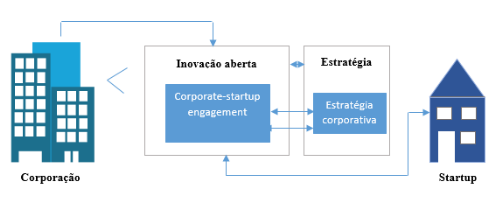
\includegraphics[]{Figuras/figura-exemplo}}
  \source{Elaborado pelo autor}
  \label{figura-exemplo}
\end{figure}

Otorrinolaringologista, Otorrinolaringologista, Otorrinolaringologista, Otorrinolaringologista, Otorrinolaringologista, Otorrinolaringologista, Otorrinolaringologista, Otorrinolaringologista, Otorrinolaringologista,Otorrinolaringologista, Otorrinolaringologista, Otorrinolaringologista, Otorrinolaringologista, Otorrinolaringologista, Otorrinolaringologista, Otorrinolaringologista, Otorrinolaringologista, Otorrinolaringologista, Otorrinolaringologista,Otorrinolaringologista, Otorrinolaringologista, Otorrinolaringologista, Otorrinolaringologista, Otorrinolaringologista, Otorrinolaringologista, Otorrinolaringologista, Otorrinolaringologista, Otorrinolaringologista, Otorrinolaringologista,Otorrinolaringologista, Otorrinolaringologista, Otorrinolaringologista, Otorrinolaringologista, Otorrinolaringologista, Otorrinolaringologista, Otorrinolaringologista, Otorrinolaringologista, Otorrinolaringologista, Otorrinolaringologista,Otorrinolaringologista, Otorrinolaringologista, Otorrinolaringologista, Otorrinolaringologista, Otorrinolaringologista, Otorrinolaringologista, Otorrinolaringologista, Otorrinolaringologista, Otorrinolaringologista, Otorrinolaringologista,Otorrinolaringologista, Otorrinolaringologista, Otorrinolaringologista, Otorrinolaringologista, Otorrinolaringologista, Otorrinolaringologista, Otorrinolaringologista, Otorrinolaringologista, Otorrinolaringologista, Otorrinolaringologista,Otorrinolaringologista, Otorrinolaringologista, Otorrinolaringologista, Otorrinolaringologista, Otorrinolaringologista, Otorrinolaringologista, Otorrinolaringologista, Otorrinolaringologista, Otorrinolaringologista, Otorrinolaringologista,Otorrinolaringologista, Otorrinolaringologista, Otorrinolaringologista, Otorrinolaringologista, Otorrinolaringologista, Otorrinolaringologista, Otorrinolaringologista, Otorrinolaringologista, Otorrinolaringologista, Otorrinolaringologista,Otorrinolaringologista, Otorrinolaringologista, Otorrinolaringologista, Otorrinolaringologista, Otorrinolaringologista, Otorrinolaringologista, Otorrinolaringologista, Otorrinolaringologista, Otorrinolaringologista, Otorrinolaringologista,Otorrinolaringologista, Otorrinolaringologista, Otorrinolaringologista, Otorrinolaringologista.

\begin{grafico}[!hbt]
  \centering
  \caption{Um gráfico de exemplo}
  \makebox[0pt]{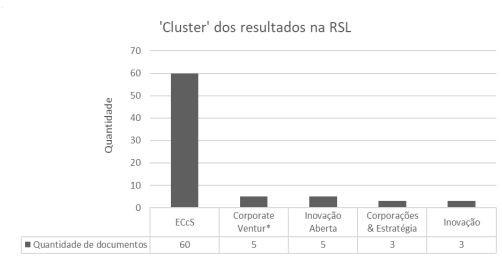
\includegraphics[]{Gráficos/grafico-exemplo}}
  \source{Elaborado pelo autor}
  \label{grafico-exemplo}
\end{grafico}
